\section{Users}
\label{sec:Users}

\begin{figure}[H]
\centering
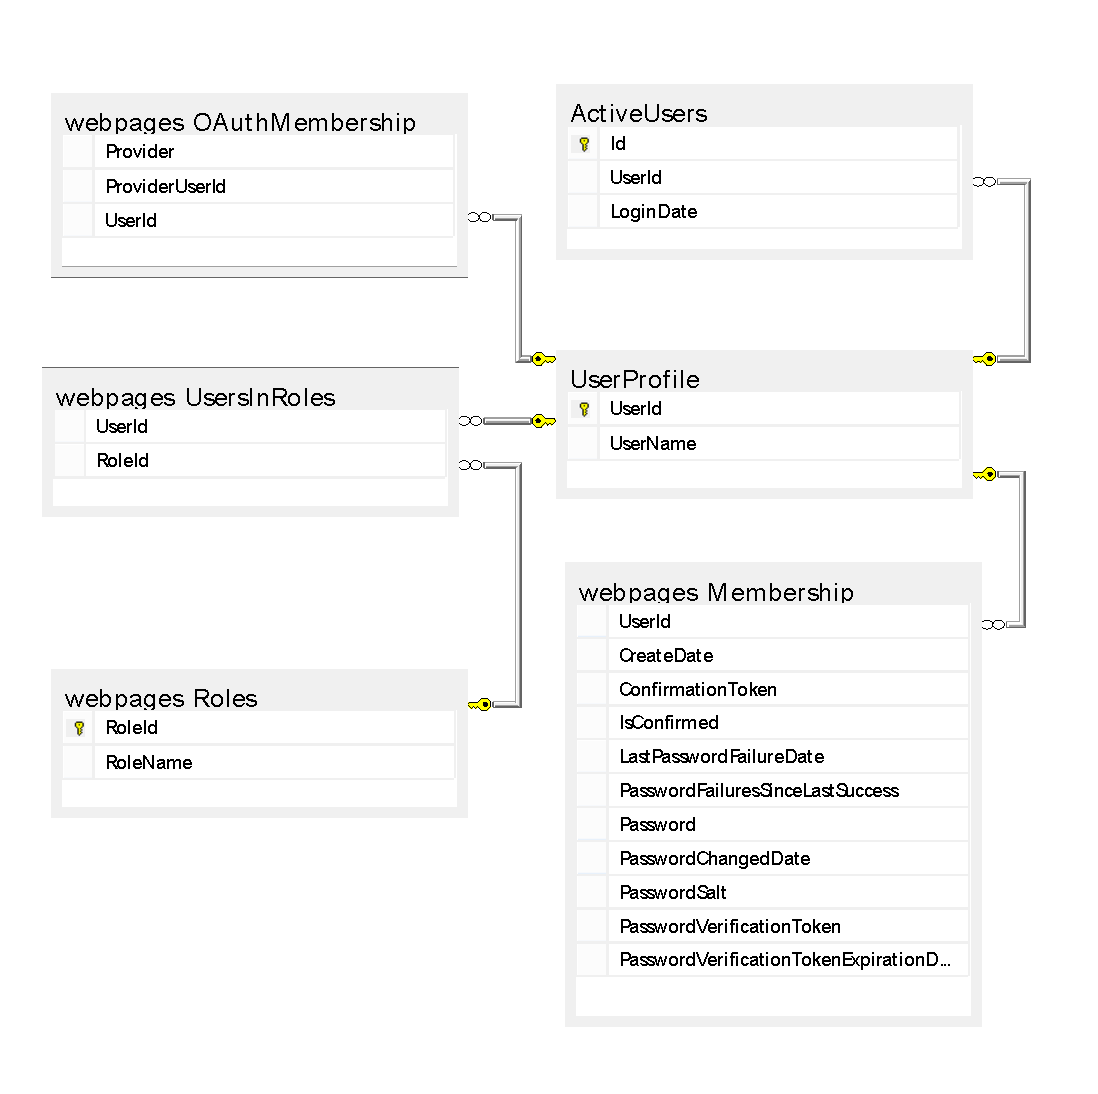
\includegraphics[width=1.0\linewidth]{./Bilder/UserEntities}
\caption{Datenbankmodell f�r Benutzerobjekte}
\label{fig:UserEntities}
\end{figure}

\subsection{MVC spezifische Tabellen}
Alle Tabellen aus dem Diagramm \ref{fig:UserEntities} mit Ausnahme der
ActiveUsers-Tabelle werden von MVC generiert und verwaltet. Sie dienen zur Benutzerauthentifizierung und zur Autorisierung. 

Relevant f�r StudMap sind die Tabellen "'webpages\_Roles"' und
"'webpages\_UserInRoles"'. Hier werden bestehenden Nutzern Rollen
zugewiesen. Um die Admin-Oberfl�che nutzen zu k�nnen, muss einem
Nutzer die Rolle "'Admin"' zugewiesen worden sein.

\subsection{ActiveUsers}
In dieser Tabelle wird festgehalten, welche Benutzer innerhalb 
eines festgelegten Zeitraums unsere App benutzt haben
Diese Tabelle kann z.B. um die letzte Position des Nutzers
erweitert werden. Dadurch k�nnten andere Nutzer sehen, wer 
gerade in ihrer N�he ist.

\begin{tabularx}{\textwidth}{|l|l|X|}
\hline \textbf{Spaltenname} & \textbf{Datentype} & \textbf{Bedeutung}  \\ 
\hline Id 					& INTEGER (PK)		 & ID des Eintrags \\ 
\hline UserId 				& INTEGER (FK)		 & ID des Nutzers \\ 
\hline LoginDate 	     	& DATETIME 			 & Zeitpunkt der letzten Anmeldung bzw. Nutzung der App\\ 
\hline 
\end{tabularx} 
